\documentclass{article} 

\usepackage[english]{babel}

\usepackage[letterpaper,top=1cm,bottom=1cm,left=3cm,right=3cm,marginparwidth=1.75cm]{geometry}

\usepackage{amsmath}
\usepackage{graphicx}
\usepackage[colorlinks=true, allcolors=blue]{hyperref}

\title{Study of IoT Architecture and Application Invariant
Functionalities}


\begin{document}
\maketitle


\end{abstract}

\section{SUMMARY}

IoT is a conjunction of many technologies and it
has spanned across diverse and multidisciplinary application
domains. Each domain has its own set of application requirements
thereby inhibiting the use of conventional programming models.
As a result there is a strong need for intermediate software
abstraction layer to hide various technological details underlying
IoT. In this paper, we propose two high level concepts of IoT,
first is the IoT architecture for systematic study of common
characteristics and second is the IoT application invariant functionalities and programming patterns. We think that our work
exposes a step forward to review on the overall IoT architecture
and provides a lightweight approach when designing software
abstraction layer with minimalist programming functionalities
that are IoT application invariant.

\section{IOT ARCHITECTURE}

Idea of ideal Internet of Things (IoT) architecture is far from reality due to the multi- and inter-disciplinary nature of IoT. For our work we decided to adopt a more simplified 4-layer architecture that allows us to capture most IoT application characteristics.

\subsection{Layer-1 - Device-Layer}

One of the characteristics of this layer is that it consists of a (large) network of heterogeneous IoT end-devices like sensor, actuator, transceiver and processing unit - that together perform the desired application task.
Selecting a particular device/hardware technology for a given application is not trivial, because of heterogeneous application, hardware and software requirements [18].
There are number of possible ways a network of IoT end systems in layer-1 can communicate with the rest of the IoT sub system as shown in Table I along with example application and technologies.
In conclusion this layer has the highest degree of heterogeneity in terms of hardware devices, software support, communication and network protocols.

\subsection{Layer-2 - Edge-Layer}

At the very least this layer act as bridge to exchange data between device-layer and cloud layer without any data manipulation but in other cases it might implement some complex cloud services which also referred to as "Fog Computing" or "Edge Computing".
The facility to port complex cloud services closer to layer-1 allows reduced bandwidth utilization and latency for critical applications.
The hardware system used in this layer is generally made up of processing unit with abundant resources to support state of the art operating systems.

\subsection{Layer-3 - Cloud-Layer}

Bulk data received from the previous layer are stored in the cloud for further processing.
This layer expose the required tools to help in the development of various cloud applications and services like visualization, analytics, cross-domain data exchange, cognitive computing, big data, machine learning algorithm and artificial intelligence (AI) to name a few.
This layer expose close to no hardware heterogeneity as IoT application developers take advantage of available cloud services like SaaS (Software as a Service), PaaS (Platform as a Service) and IaaS (Infrastructure as a Service) from various service providers like Amazon, Google, Microsoft, etc.

\subsection{IoT Cross-Layer Management}

Provisioning for system management helps in the deployment and maintenance of IoT end-system and is also considered an important requirement from business point of view .
There can be many possibilities for inter- and intra-layer communication depending on the producer and consumer of data.
Finally, in contrast to existing work, the architecture discussed in this section highlights the common characteristics observed in various application domains which is useful for understanding and developing various functionalities of IoT and also it introduces an important system management cross-layer for deployment and maintenance of IoT systems.



\section{IoT Application Invariant Functionality (IF) and Programming Pattern (PP)}

\begin{document}
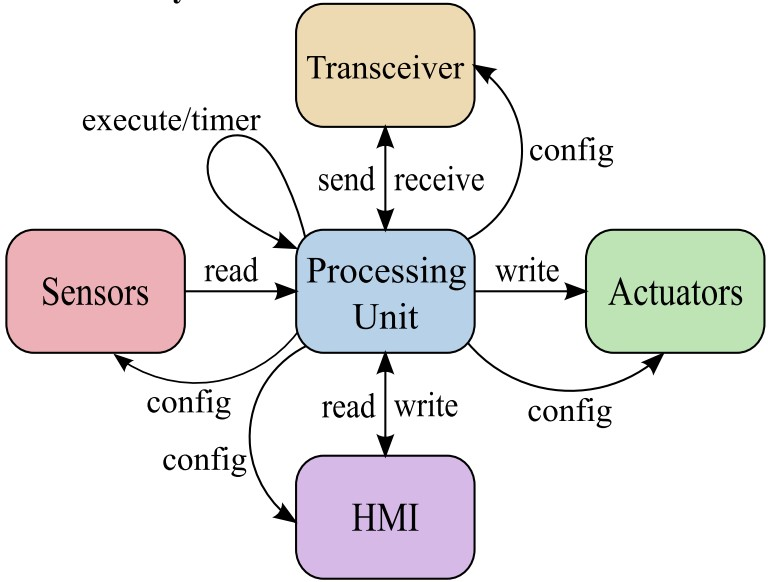
\includegraphics[width=0.3\textwidth]{End system.jpg}
\caption{\label{fig:End system}}


\subsection{Layer-1 IF and PP}

Irrespective of IoT domain and its requirements an IoT end-system performs some basic high-level invariant functions as explained hereafter .
These functions are programmed in the memory of processing unit (PU) and is responsible for controlling the behavior of other IoT end-devices.
We observed that an application code for IoT end-system follows some basic programming patterns .
These programming patterns can be easily visualized as finite-state machine, where each state is one of the basic operation performed by processing unit along with respective inter-layer communication.

\begin{document}
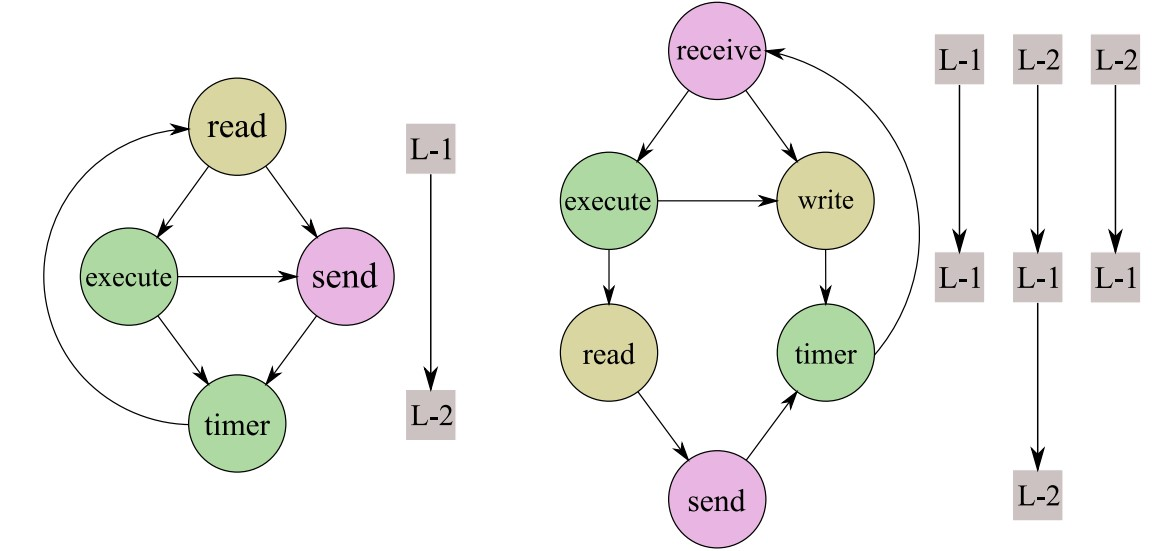
\includegraphics[width=0.4\textwidth]{Layer1.jpg}
\caption{ }



\subsection{Layer-2 IF and PP}

The network of gateways at this layer consists of two sets of send and receive functions, the first set of functions is used to exchange data from layer-1using the available low power wireless communication (LR-WPAN or LPWAN) and the second set of functions is for the Internet backhaul using standard wired or wireless communication protocol like 3GPP/4G, LTE, WLAN, etc.
One of the important feature of this layer is the capabilty to execute relevant cloud services closer to layer-1, therefore a gateway can expose a high level execute command that a user can bind to one or more services.
We have observed that a gateway follows a very simple programming pattern to communicate with layer-1 and layer-2

\begin{document}
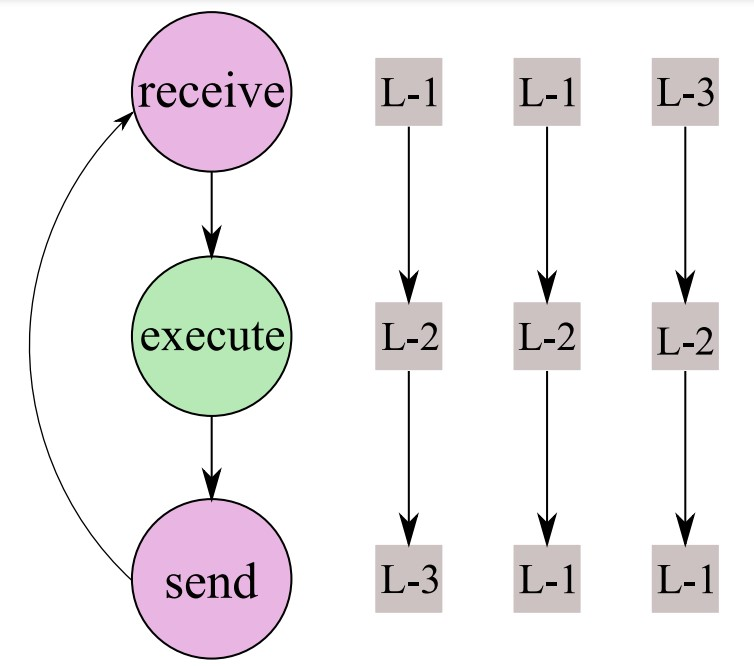
\includegraphics[width=0.3\textwidth]{Layer 2.jpg}
\caption{ }



\subsection{Layer-3 IF and PP}

Similar to layer-1 and layer-2 this layer also consists of send and receive functions to exchange data with layer-2 or directly with layer-1 bypassing gateway.
The most important feature is to execute various cloud services and configure the cloud instances on demand.
Cross-Layer IF and PP - Most of the challenges related to cross-layer functionalities relates to orchestrating the deployment and behavior of devices application logic, maintaining the status of their firmware version and monitoring the data exchanged even in case of network failure.


\bibliography{sample}

\end{document}
